\documentclass[convert={outext=.tex.png}]{standalone}
\usepackage{ulem,tikz,xcolor}
\usetikzlibrary{arrows,arrows.meta,calc,fit,positioning,shapes,shapes.geometric}

\tikzset{database/.style={draw,cylinder,aspect=0.5,shape border rotate=90}}

\begin{document}
\pagecolor[RGB]{255,255,254}
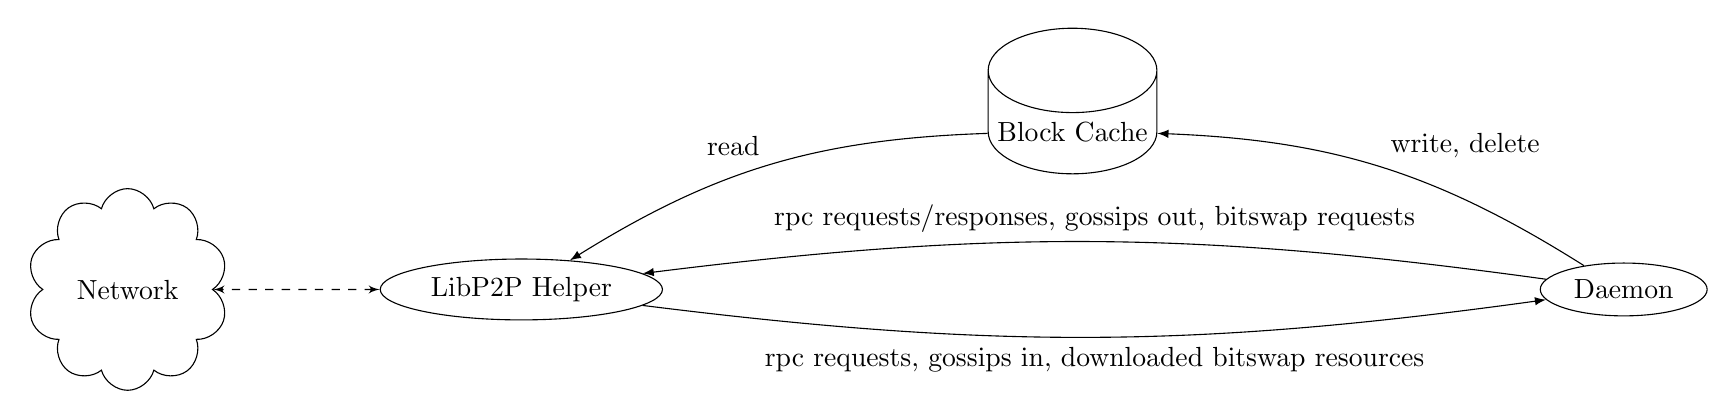
\begin{tikzpicture}
  \node[database] (db) at (0,0) {Block Cache};
  \node[draw,ellipse] (helper) at (-7,-2) {LibP2P Helper};
  \node[draw,ellipse] (daemon) at (7,-2) {Daemon};
  \node[draw,cloud,cloud puffs=10] (network) at (-12, -2) {Network};

  \draw[-latex] (daemon) to[bend right=15] node[above right] {write, delete} (db);
  \draw[-latex] (db) to[bend right=15] node[above left] {read} (helper);
  \draw[-latex] (helper) to[bend right=7.5] node[below] {rpc requests, gossips in, downloaded bitswap resources} (daemon);
  \draw[-latex] (daemon) to[bend right=7.5] node[above] {rpc requests/responses, gossips out, bitswap requests} (helper);
  \draw[latex'-latex',dashed] (helper) -- (network);
\end{tikzpicture}
\end{document}
